\section{Análise de Redes}
    
    \vspace{10.5cm}
    
    \hspace{1cm}
    A rede mundial de computadores é a ferramenta mais usada para disseminar informações. Entretanto, também possibilita diversas formas de ataques a hospedeiros vulneráveis. Entendemos por incidente um ataque ocorrido, seja ele decorrente de uma tentativa de intrusão, seja ele um evento anômalo ocorrido em uma rede interna. De qualquer forma, é necessário gerar uma resposta, para que ele não se repita e os danos causados sejam reduzidos. Para isso, precisamos analisar os vestígios digitais da rede em que sistemas finais envolvidos estão introduzidos.
    
    \vspace{4mm}
    
    \hspace{1cm}
    Para analisar artefatos digitais em uma rede, precisamos relembrar os conceitos apresentados nas seções \ref{cap1_ir} e \ref{cap1_visao_geral}. Na etapa de análise dos dados no processo de Resposta a Incidentes, é importante considerar informações de rede providas de dispositivos de acesso à \textit{Internet}, interfaces de serviços terceirizados na nuvem, sistemas de detecção de intrusão, entre outros \cite{luttgens2014}, porém, a simples aquisição desses dados não é suficiente para auxiliar uma investigação. Consequentemente, faz-se necessária a presença do ser humano para fornecer um contexto para os dados, de uma investigação, colocados em evidência.
    
    \subsection{Técnicas}
    
    \hspace{1cm}
    A técnica denominada \textit{packet sniffing} é amplamente usada para coletar pacotes de rede. O especialista configura um receptor passivo para copiar os dados que trafegam por determinado canal de comunicação \cite{kurose2013}. Em seguida, filtra estes dados, por pacotes referentes a hospedeiros e processos específicos, e os analisa.
    
    \vspace{4mm}
    
    \hspace{1cm}
    Existem bases de dados que armazenam informações aproximadas da geolocalização atual de um endereço IP da \textit{Internet}. A técnica denominada \textit{IP lookup} pode ser empregada por meio da utilização de sites que disponibilizam uma base de dados de IPs para consulta. Como exemplo, o site \href{https://www.ip-lookup.org/}{https://www.ip-lookup.org/}. 
    
    \subsection{Ferramentas} \label{cap4_ferramentas}

    \hspace{1cm}
    A ferramenta \textit{whois} fornece informações de registro de domínio de um endereço IP da \textit{Internet}. Sites como o do \href{https://registro.br/tecnologia/ferramentas/whois/}{Registro.br} podem ser usados para consultar tais informações.

    \vspace{4mm}

    \hspace{1cm}
    Organizações dispõem de \textit{Firewalls} e sistemas de detecção de intrusão (do inglês IDS ou \textit{intrusion detection system}), para tentar proteger sua rede contra ataques. Estes, notificam administradores de rede sobre a quebra de alguma política de acesso \cite{bejtlich2004}. Aqueles bloqueiam tentativas de conexão partidas de hospedeiros externos que estejam enviando pacotes para uma porta específica de um serviço.
    
    \vspace{4mm}
    
    \hspace{1cm}
    Como \textit{Firewalls} não conseguem detectar anomalias originadas pela rede interna de uma empresa, complementa-se sua utilização com os IDS. Entretanto, as ameaças mudam com o tempo, e essas ferramentas não conseguem detectar novas formas de intrusão, apenas conhecidas \cite{capobianco2019}.

    \vspace{4mm}

    \hspace{1cm}
    A filtragem pelos dados desejados pode ser feita por meio da biblioteca \textit{libpcap}. Ela é utilizada por ferramentas de captura e análise de redes, como \textit{tcpdump} e \textit{Wireshark} \cite{bejtlich2004}. Ao contrário da primeira, a segunda apresenta os pacotes trafegados na rede por meio de uma interface gráfica, como mostra a figura \ref{wireshark_ex}. 
    
    \begin{figure}[H]
    	\centering
    	\caption{Interface gráfica da Wireshark}
    	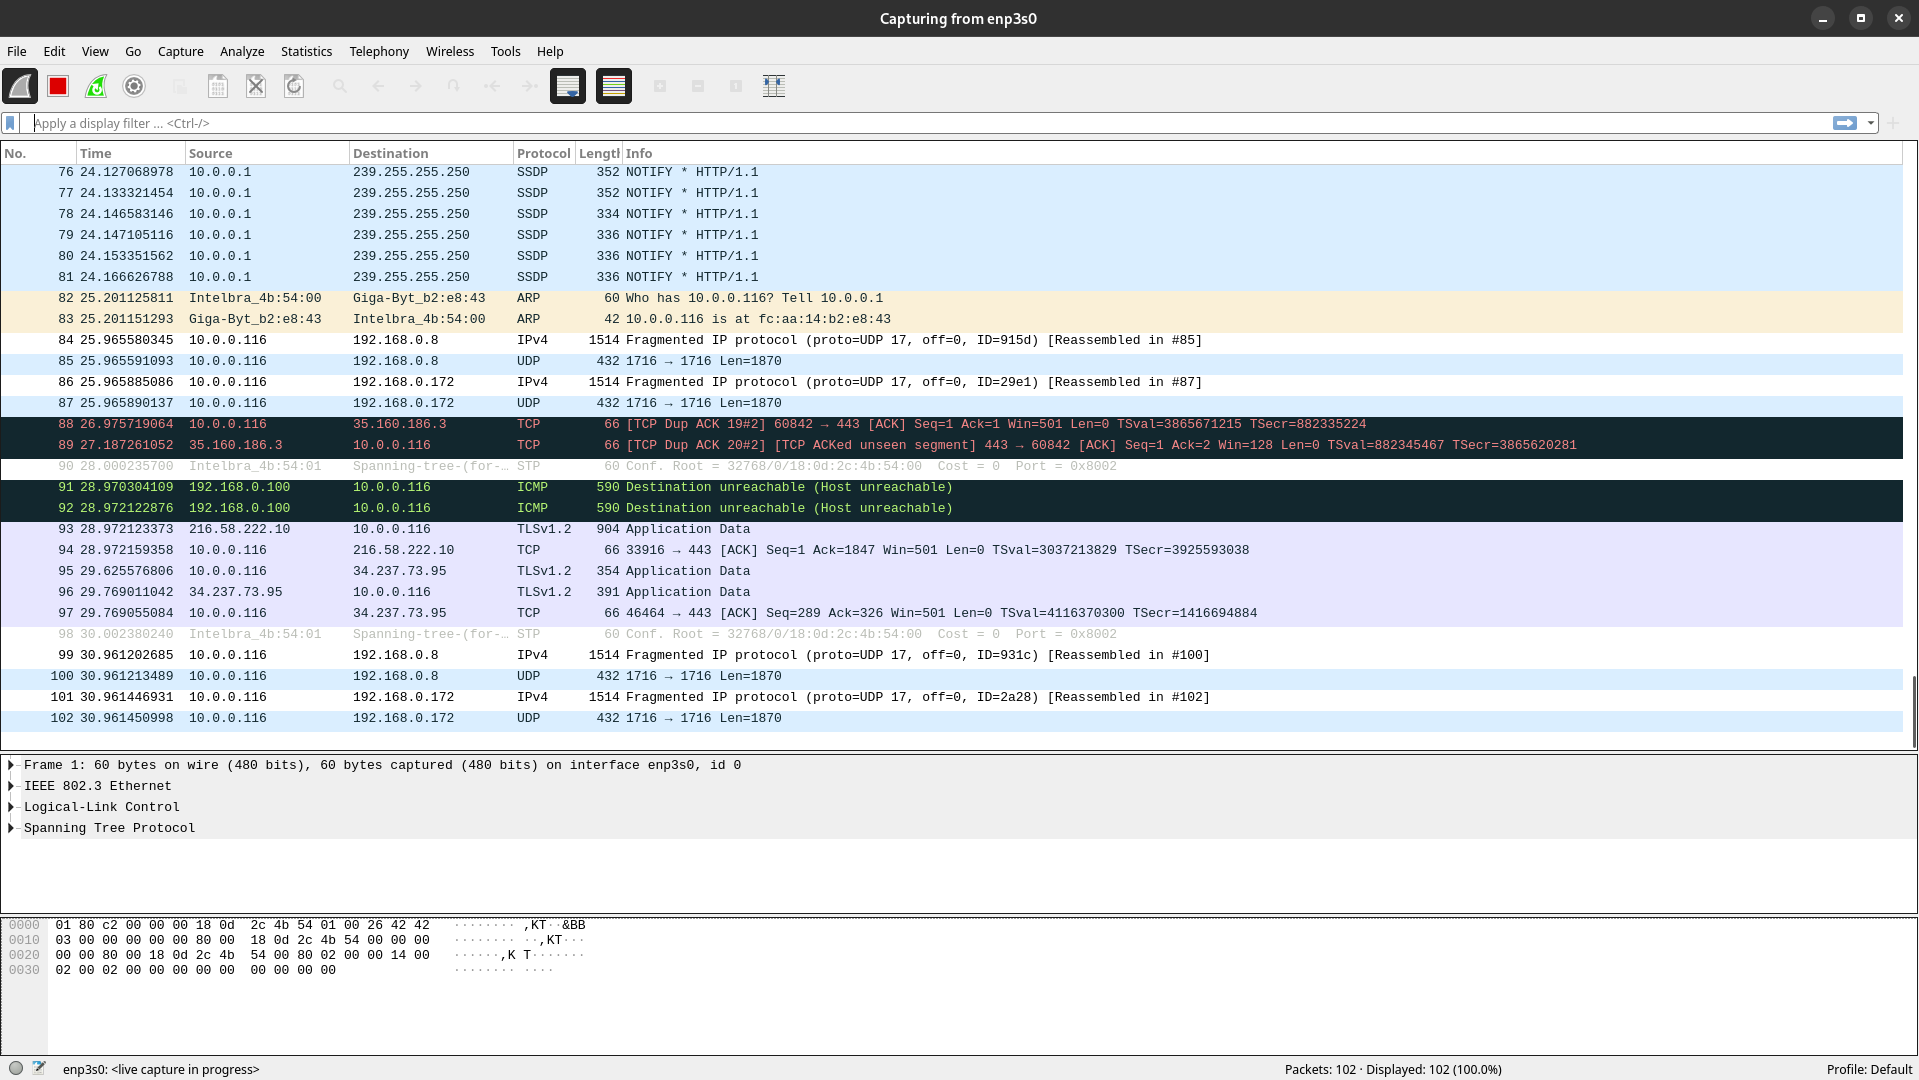
\includegraphics[scale=0.28]{img_wireshark}
    	\caption*{Fonte: o próprio autor.}
    	\label{wireshark_ex}
    \end{figure}

    \hspace{1cm}
    Em suma, para responder a um incidente, o profissional deve ter identificado todas as vulnerabilidades da rede, oriundas de hospedeiros comprometidos. Para tentar garantir a não reincidência de um ataque, sistemas IDS devem ser atualizados, para abranger falhas internas. Também, \textit{Firewalls} devem ser corrigidos para barrar acessos externos indesejados. Por fim, esses sistemas são mantidos por especialistas de rede, que realiza análise de pacotes e de logs de rede.

    \subsection{Exercícios}
    
    \begin{example}[\quad \large Análise de Redes] \label{cap4_exercicios}
        \begin{enumerate}
            \item O que um perito deveria fazer, caso quisesse interceptar pacotes trocados por dois hospedeiros distintos na rede ?
            \item Explique a diferença entre \textit{Firewall} e sistemas de detecção de intrusão (IDS).
            \item Ao identificar o endereço IP de origem de um pacote de rede, é possível tentar localizar o hospedeiro no globo terrestre ? 
            \item Escolha um site na \textit{Internet} e consulte suas informações de domínio em \href{https://registro.br/tecnologia/ferramentas/whois/}{Registro.br}. Em seguida, 
            liste informações sobre os supostos proprietários de tal domínio.
        \end{enumerate}
    \end{example}

\newpage